% \iffalse
%<*internal|cls|sty>
\def\Version{2021/01/31 v1.1.1}
%</internal|cls|sty>
%<*internal>
\iffalse
%</internal>
%<cls|sty>\NeedsTeXFormat{LaTeX2e}[2005/12/01]
%<*cls&letter>
\ProvidesClass{hu-berlin-letter}
  [\Version\ Humboldt-Universit"at zu Berlin - letter documentclass]
\ClassInfo{hu-berlin}{* * * hu-berlin * * *\MessageBreak
    Part of the hu-berlin Bundle }
%</cls&letter>
%<*sty>
%<*style>
\ProvidesPackage{hu-berlin-bundle-style}
  [\Version\space hu-berlin - package for style the documentation]
  \PackageInfo{hu-berlin}{* * * hu-berlin * * *\MessageBreak
	  Part of the hu-berlin Bundle}
%</style>
%<*base>
\ProvidesPackage{hu-berlin-base}
  [\Version\space hu-berlin - package for basic features]
  \PackageInfo{hu-berlin}{* * * hu-berlin * * *\MessageBreak
	  Part of the hu-berlin Bundle}
%</base>
%</sty>
%<*driver>
\catcode9=12
\ProvidesFile{\jobname.dtx}
	[\Version\space Documentation of the hu-berlin Bundle]
%</driver>
% /*
%       ██████  ███████  █████  ██████  ███    ███ ███████
% ▄ ██ ▄██   ██ ██      ██   ██ ██   ██ ████  ████ ██
%  ████ ██████  █████   ███████ ██   ██ ██ ████ ██ █████
% ▀ ██ ▀██   ██ ██      ██   ██ ██   ██ ██  ██  ██ ██
%       ██   ██ ███████ ██   ██ ██████  ██      ██ ███████
% */
%<*readme&main>
hu-berlin-bundle
================

This package provides files according to the corporate design
for the Humboldt-Universität zu Berlin.
It is _no_ official package of the university itself and
not officially approved by it.

You find more information in the official [corporate design guideline](https://www.hu-berlin.de/de/hu-intern/design/basiselemente/leitfaden-corporate-design-hu.pdf) 
and on the website <https://www.hu-berlin.de/de/hu-intern/design>.

## Documents and Documentations for hu-berlin bundle


This bundle provides following files:

  * `hu-berlin-bundle.dtx` which is the core file designed with literate programming 
  * `hu-berlin-bundle.ins` which is the installation file for all necessary files generated automatically
  * `hu-berlin-bundle.pdf` is documentation of the bundle.
  * `README.md`
  * `makefile`

All other files can and will be generated from the `.dtx` file (see below).

Furthermore there is the folder `img` which contains the necessary image files.


This work has the LPPL maintenance status _maintained_.
The current maintainer of this work is [Lukas C. Bossert](https://github.com/lukascbossert).


You find this bundle versioned and available on [Zenodo](https://doi.org/10.5281/zenodo.3251728) 

%</readme&main>
% /*
%     ██ ██████  ███████  █████  ██████  ███    ███ ███████
%    ██  ██   ██ ██      ██   ██ ██   ██ ████  ████ ██
%   ██   ██████  █████   ███████ ██   ██ ██ ████ ██ █████
%  ██    ██   ██ ██      ██   ██ ██   ██ ██  ██  ██ ██
% ██     ██   ██ ███████ ██   ██ ██████  ██      ██ ███████
% */
% /*
%       ██████  ██ ██████
% ▄ ██ ▄██   ██ ██ ██   ██
%  ████ ██████  ██ ██████
% ▀ ██ ▀██   ██ ██ ██   ██
%       ██████  ██ ██████
% */
%<*bib>
%%
%% Encoding: UTF-8
%%
@InCollection{Hoare1973,
  author = {Charles Antony Richard Hoare},
  title = {Hints on programming language design},
  editor = {C. Bunyan},
  booktitle = {Computer Systems Reliability},
  series = {State of the Art Report},
  number = {20},
  pages = {193--216},
  date = {1973},
  url={http://flint.cs.yale.edu/cs428/doc/HintsPL.pdf},
  urldate={2018-09-06},
  comment = {\blockcquote[195]{Hoare1973}{Documentation must be regarded as an integral part of the process of design and coding.
 A good programming language will encourage and assist the programmer to write clear,
 self-documenting code,
 and even perhaps to develop
 and display a pleasant style
 of writing.}}
}

%</bib>
% /*
%     ██ ██████  ██ ██████
%    ██  ██   ██ ██ ██   ██
%   ██   ██████  ██ ██████
%  ██    ██   ██ ██ ██   ██
% ██     ██████  ██ ██████
% */
%<*internal>
\fi
\def\nameofplainTeX{plain}
\ifx\fmtname\nameofplainTeX\else
  \expandafter\begingroup
\fi
%</internal>
% /*
%        ██ ███    ██ ███████
% ▄ ██ ▄██ ████   ██ ██
%  ████ ██ ██ ██  ██ ███████
% ▀ ██ ▀██ ██  ██ ██      ██
%        ██ ██   ████ ███████
% */
%<*install>
%% \CharacterTable
%%  {Upper-case    \A\B\C\D\E\F\G\H\I\J\K\L\M\N\O\P\Q\R\S\T\U\V\W\X\Y\Z
%%   Lower-case    \a\b\c\d\e\f\g\h\i\j\k\l\m\n\o\p\q\r\s\t\u\v\w\x\y\z
%%   Digits        \0\1\2\3\4\5\6\7\8\9
%%   Exclamation   \!     Double quote  \"     Hash (number) \#
%%   Dollar        \$     Percent       \%     Ampersand     \&
%%   Acute accent  \'     Left paren    \(     Right paren   \)
%%   Asterisk      \*     Plus          \+     Comma         \,
%%   Minus         \-     Point         \.     Solidus       \/
%%   Colon         \:     Semicolon     \;     Less than     \<
%%   Equals        \=     Greater than  \>     Question mark \?
%%   Commercial at \@     Left bracket  \[     Backslash     \\
%%   Right bracket \]     Circumflex    \^     Underscore    \_
%%   Grave accent  \`     Left brace    \{     Vertical bar  \|
%%   Right brace   \}     Tilde         \~}

\input docstrip.tex
\keepsilent
\askforoverwritefalse

\nopreamble\nopostamble

\usedir{doc/latex/\jobname}
\generate{
  \file{README.md}{\from{\jobname.dtx}{readme,main}}
  \file{hu-berlin-bundle-bibliography.bib}{\from{\jobname.dtx}{bib}}
  \file{hu-berlin-letter-example-lualatex.tex}{\from{\jobname.dtx}{example,letter}}
  \file{hu-berlin-letter-example-markdown.md}{\from{\jobname.dtx}{example,letter-md}}
}

\preamble
----------------------------------------------------------------
hu-berlin-bundle
Author:  Lukas C. Bossert
E-mail:  lukas@texografie.de
License: Released under the LaTeX Project Public License v1.3c or later
See:     http://www.latex-project.org/lppl.txt
Various parts my have a different licence,
please consider and respect them carefully.
----------------------------------------------------------------

\endpreamble
\postamble
 
Copyright (C) 2019-2020
\endpostamble

\usedir{tex/latex/\jobname}
\generate{
  \file{hu-berlin-letter-example-lualatex.tex}{\from{\jobname.dtx}{example,letter}}
  \file{hu-berlin-letter-example.lco}{\from{\jobname.dtx}{example,lco}}
  \file{hu-berlin-letter.cls}{\from{\jobname.dtx}{cls,letter}}
  %
  \file{hu-berlin-base.sty}{\from{\jobname.dtx}{sty,base}}
  \file{hu-berlin-bundle-style.sty}{\from{\jobname.dtx}{sty,style}}
  \file{hu-berlin-letter-template.latex}{\from{\jobname.dtx}{template,letter-md}}
}
%</install>
%<install>\endbatchfile
%<*internal>
\usedir{source/latex/\jobname}
\generate{
  \file{\jobname.ins}{\from{\jobname.dtx}{install}}
}
\ifx\fmtname\nameofplainTeX
  \expandafter\endbatchfile
\else
  \expandafter\endgroup
\fi
%</internal>
% /*
%     ██ ██ ███    ██ ███████
%    ██  ██ ████   ██ ██
%   ██   ██ ██ ██  ██ ███████
%  ██    ██ ██  ██ ██      ██
% ██     ██ ██   ████ ███████
% */
%<*driver>
\ProvidesFile{\jobname.dtx}
	[\Version\space Documents and documentation for hu-berlin]
%</driver>
% /*
% ██████   ██████   ██████  ██████ ██       █████  ███████ ███████
% ██   ██ ██    ██ ██      ██      ██      ██   ██ ██      ██
% ██   ██ ██    ██ ██      ██      ██      ███████ ███████ ███████
% ██   ██ ██    ██ ██      ██      ██      ██   ██      ██      ██
% ██████   ██████   ██████  ██████ ███████ ██   ██ ███████ ███████
% */
%<*driver>
\def\huberlinsubject{Guideline}
\def\huberlinshort{hu-berlin-bundle}
\def\huberlintitle{%
Documents and Documentations for \LaTeX\ at the Humboldt-Universität zu Berlin (unofficial)}
\def\huberlinsubtitle{For Authors and Developers}
\def\huberlinauthor{Lukas C. Bossert}
\RequirePackage{scrlfile}
\PassOptionsToClass{%
	english
   ,oneside
  }{scrbook}
\ReplaceClass{article}{scrbook}
\documentclass{ltxdoc}
\usepackage{hu-berlin-bundle-style} 
\GetFileInfo{\jobname.dtx}
% /*
%           ██████   ██████   ██████ ██    ██ ███    ███ ███████ ███    ██ ████████
% ▄ ██ ▄    ██   ██ ██    ██ ██      ██    ██ ████  ████ ██      ████   ██    ██
%  ████     ██   ██ ██    ██ ██      ██    ██ ██ ████ ██ █████   ██ ██  ██    ██
% ▀ ██ ▀    ██   ██ ██    ██ ██      ██    ██ ██  ██  ██ ██      ██  ██ ██    ██
%           ██████   ██████   ██████  ██████  ██      ██ ███████ ██   ████    ██
% */
\begin{document}
\openoutputfile{\jobname.pkglist}{pkglist}
\pdfbookmark[section]{\contentsname}{toc}
\tableofcontents
\clearpage
\chapter{Introduction}
\begin{markdown*}{hybrid=true}
%</driver>
% /*
%       ██████  ███████  █████  ██████  ███    ███ ███████
% ▄ ██ ▄██   ██ ██      ██   ██ ██   ██ ████  ████ ██
%  ████ ██████  █████   ███████ ██   ██ ██ ████ ██ █████
% ▀ ██ ▀██   ██ ██      ██   ██ ██   ██ ██  ██  ██ ██
%       ██   ██ ███████ ██   ██ ██████  ██      ██ ███████
% */
%<*readme,main>

With this (unofficial) bundle you have several documents which are designed according to the corporate design of the Humboldt-Universität zu Berlin.


Following documents or documentclasses are available:

* letter (`hu-berlin-letter.cls`); via `.tex` and `.md`
* base package (`hu-berlin-base.sty`)


## Installation of the bundle
`hu-berlin` is part of the distributions [MiKTeX](http://www.miktex.org)
and [TeXLive](http://www.tug.org/texlive) -- thus, you
can easily install it using the respective package manager.
If you would like to
install `hu-berlin-bundle` into your local folder  manually, do the following:
Go to your terminal, browse to the folder of this bundle and run

```
make install
```


If you are using macOS you might be asked for your user account password for the installation.


Further options of this makefile are:

* `clean`:  deletes all unnecessary files
* `cleanbundle`:  deletes all files except `.dtx`, `.md`. You will get the plain version of this bundle.
This might be helpful if you send the bundle to someone else.
* `ctan`:  this will create a zip file which can be used to send to CTAN.
* `files`: will only create the files from the `.dtx`-scratch.
* `uninstall`: will erase the locally installed files.


This bundle is constantly updated. For hints, errors or suggestions use the GitHub repository [https://github.com/LukasCBossert/hu-berlin-bundle](https://github.com/LukasCBossert/hu-berlin-bundle).

## Changelog

All notable changes to this project will be documented in the [README.md](https://github.com/LukasCBossert/hu-berlin-bundle/blob/master/README.md).
This project **does not** adhere to [Semantic Versioning](http://semver.org/).
The markdown syntax is inspired by the conventions proposed by [keepachangelog.com](http://keepachangelog.com/).

### v1.1.1 (2021/01/31)
* (letter) fix for language switch when using markdown-pandoc-conversion workflow 


### v1.1.0 (2021/01/31)
* (letter) language option now available also for the markdown-pandoc-conversion-workflow.

### v1.0.9 (2021/01/10)
* (letter) making everything multi-lingual (at least German and English); German is default language. You can load English e.g. by `documentclass[english]{hu-berlin-letter}` (addresses [issue No. 3](https://github.com/LukasCBossert/hu-berlin-bundle/issues/3))


### v1.0.8 (2020/10/30)
* (letter) replacing actual logo with a dummy text (due to possible copyright conflicts). 
  The correct logo has to be called `hu-berlin-logo.pdf` 
  and needs to be put somewhere in PATH so it will be found.
  If such file cannot be found a dummy text will be taken instead (`Humboldt-Universität zu Berlin´)


### v1.0.7 (2020/10/29)
* (letter) fixed missing `\removereffields`
* (letter) added missing suffix for hu-logo (`.pdf`)



### v1.0.6 (2020-10-22)
* (letter) changed address separator
* (letter) fixed empty minipage when no metadata given 
* (letter) changed default backaddress


### v1.0.5 (2020-04-28)
* (general) Changed logo format to `.pdf` 
* (letter) Changed `\ifkomavarempty` to `\ifkomavarempty`, fixes 
  [github-issue nr. 1](https://github.com/LukasCBossert/hu-berlin-bundle/issues/1)


### v1.0.4 (2019-12-19)
* Added `hu-berlin-base.sty` as a package which contains all relevant code for documents and documentclasses of the bundle.

### v1.0.3 (2019-06-26)
 * Changed the main font for compatibility with UNIX-systems (TeX Gyre Heros instead of Verdana).
 
### v1.0.2 (2019-06-22)
 Renaming files for CTAN compatability.


### v1.0.1 (2019-06-21)
 Internal changes for publishing. Still one documentclass for a letter.

### v1.0.0 (2019-06-21)
 First release with a documentclass for letter.

## Copyright
Various parts of this bundle have different copyrights.
If not otherwise stated the copyright is [The LaTeX project public license (LPPL), version 1.3c](https://www.latex-project.org/lppl/lppl-1-3c/)


### Boilerplate / markdown-template
The template for the markdown conversion, 
forked from the pandoc-templates and [JensErat pandoc-scrlttr2](https://github.com/JensErat/pandoc-scrlttr2) is dual-licensed, 
under both the GPL (v2 or higher, same as pandoc) and the BSD 3-clause license (included below).

----

Copyright (c) 2014, John MacFarlane\\  
Copyright (c) 2014, Jens Erat\\  
All rights reserved.  

Redistribution and use in source and binary forms, with or without
modification, are permitted provided that the following conditions are met:

*  Redistributions of source code must retain the above copyright notice, this list of conditions and the following disclaimer.

* Redistributions in binary form must reproduce the above copyright notice, this list of conditions and the following disclaimer in the documentation and/or other materials provided with the distribution.

* Neither the name of John MacFarlane nor the names of other contributors may be used to endorse or promote products derived from this software without specific prior written permission.

THIS SOFTWARE IS PROVIDED BY THE COPYRIGHT HOLDERS AND CONTRIBUTORS
"AS IS" AND ANY EXPRESS OR IMPLIED WARRANTIES, INCLUDING, BUT NOT
LIMITED TO, THE IMPLIED WARRANTIES OF MERCHANTABILITY AND FITNESS FOR
A PARTICULAR PURPOSE ARE DISCLAIMED. IN NO EVENT SHALL THE COPYRIGHT
OWNER OR CONTRIBUTORS BE LIABLE FOR ANY DIRECT, INDIRECT, INCIDENTAL,
SPECIAL, EXEMPLARY, OR CONSEQUENTIAL DAMAGES (INCLUDING, BUT NOT
LIMITED TO, PROCUREMENT OF SUBSTITUTE GOODS OR SERVICES; LOSS OF USE,
DATA, OR PROFITS; OR BUSINESS INTERRUPTION) HOWEVER CAUSED AND ON ANY
THEORY OF LIABILITY, WHETHER IN CONTRACT, STRICT LIABILITY, OR TORT
(INCLUDING NEGLIGENCE OR OTHERWISE) ARISING IN ANY WAY OUT OF THE USE
OF THIS SOFTWARE, EVEN IF ADVISED OF THE POSSIBILITY OF SUCH DAMAGE.
%</readme,main>
% /*
%     ██ ██████  ███████  █████  ██████  ███    ███ ███████
%    ██  ██   ██ ██      ██   ██ ██   ██ ████  ████ ██
%   ██   ██████  █████   ███████ ██   ██ ██ ████ ██ █████
%  ██    ██   ██ ██      ██   ██ ██   ██ ██  ██  ██ ██
% ██     ██   ██ ███████ ██   ██ ██████  ██      ██ ███████
% */
%<*driver>
\end{markdown*}
\clearpage
\chapter{Preambel}

This bundle consists of various files
which are either generated by the core file (|.dtx|)
or are part of the basic structure of this bundle.
You can easily pick up the basic file structure from \cref{hu-berlin:bundle-structure}.

\begin{figure}[!htb]
\footnotesize
\dirtree{%
.1 \huberlinFolder hu-berlin-bundle.
.2 hu-berlin-bundle.dtx \DTcomment{code and documentation}.
.2 hu-berlin-bundle.pdf \DTcomment{documentation}.
.2 hu-berlin-base.sty \DTcomment{basic components of the bundle}.
.2 hu-berlin-letter-example-lualatex.tex \DTcomment{letter}.
.2 hu-berlin-letter-example.lco \DTcomment{datafile for letter}.
.2 hu-berlin-letter-example-lualatex.pdf \DTcomment{letter}.
.2 hu-berlin-letter-example-markdown.pdf \DTcomment{converted letter from markdown}.
.2 hu-berlin-letter-example-markdown.md \DTcomment{example markdown file }.
.2 hu-berlin-letter-template.latex \DTcomment{template for conversion}.
.2 \huberlinFolder img\DTcomment{folder for images}.
.3 texografie-logo.pdf\DTcomment{logo of maintainer}.
.2 makefile\DTcomment{makefile to generate all required files}.
.2 README.md\DTcomment{README file with information on installation}.
}
\caption{Structure of \texttt{hu-berlin} bundle}
\label{hu-berlin:bundle-structure}
\end{figure}

When you run the |makefile|
you get all these various files described above.




\DocInput{\jobname.dtx}

\printbibliography


\part{Example files}
\chapter{Letter}
\section{From \texttt{.tex}}
\IfFileExists{hu-berlin-letter-example-lualatex.pdf}
  {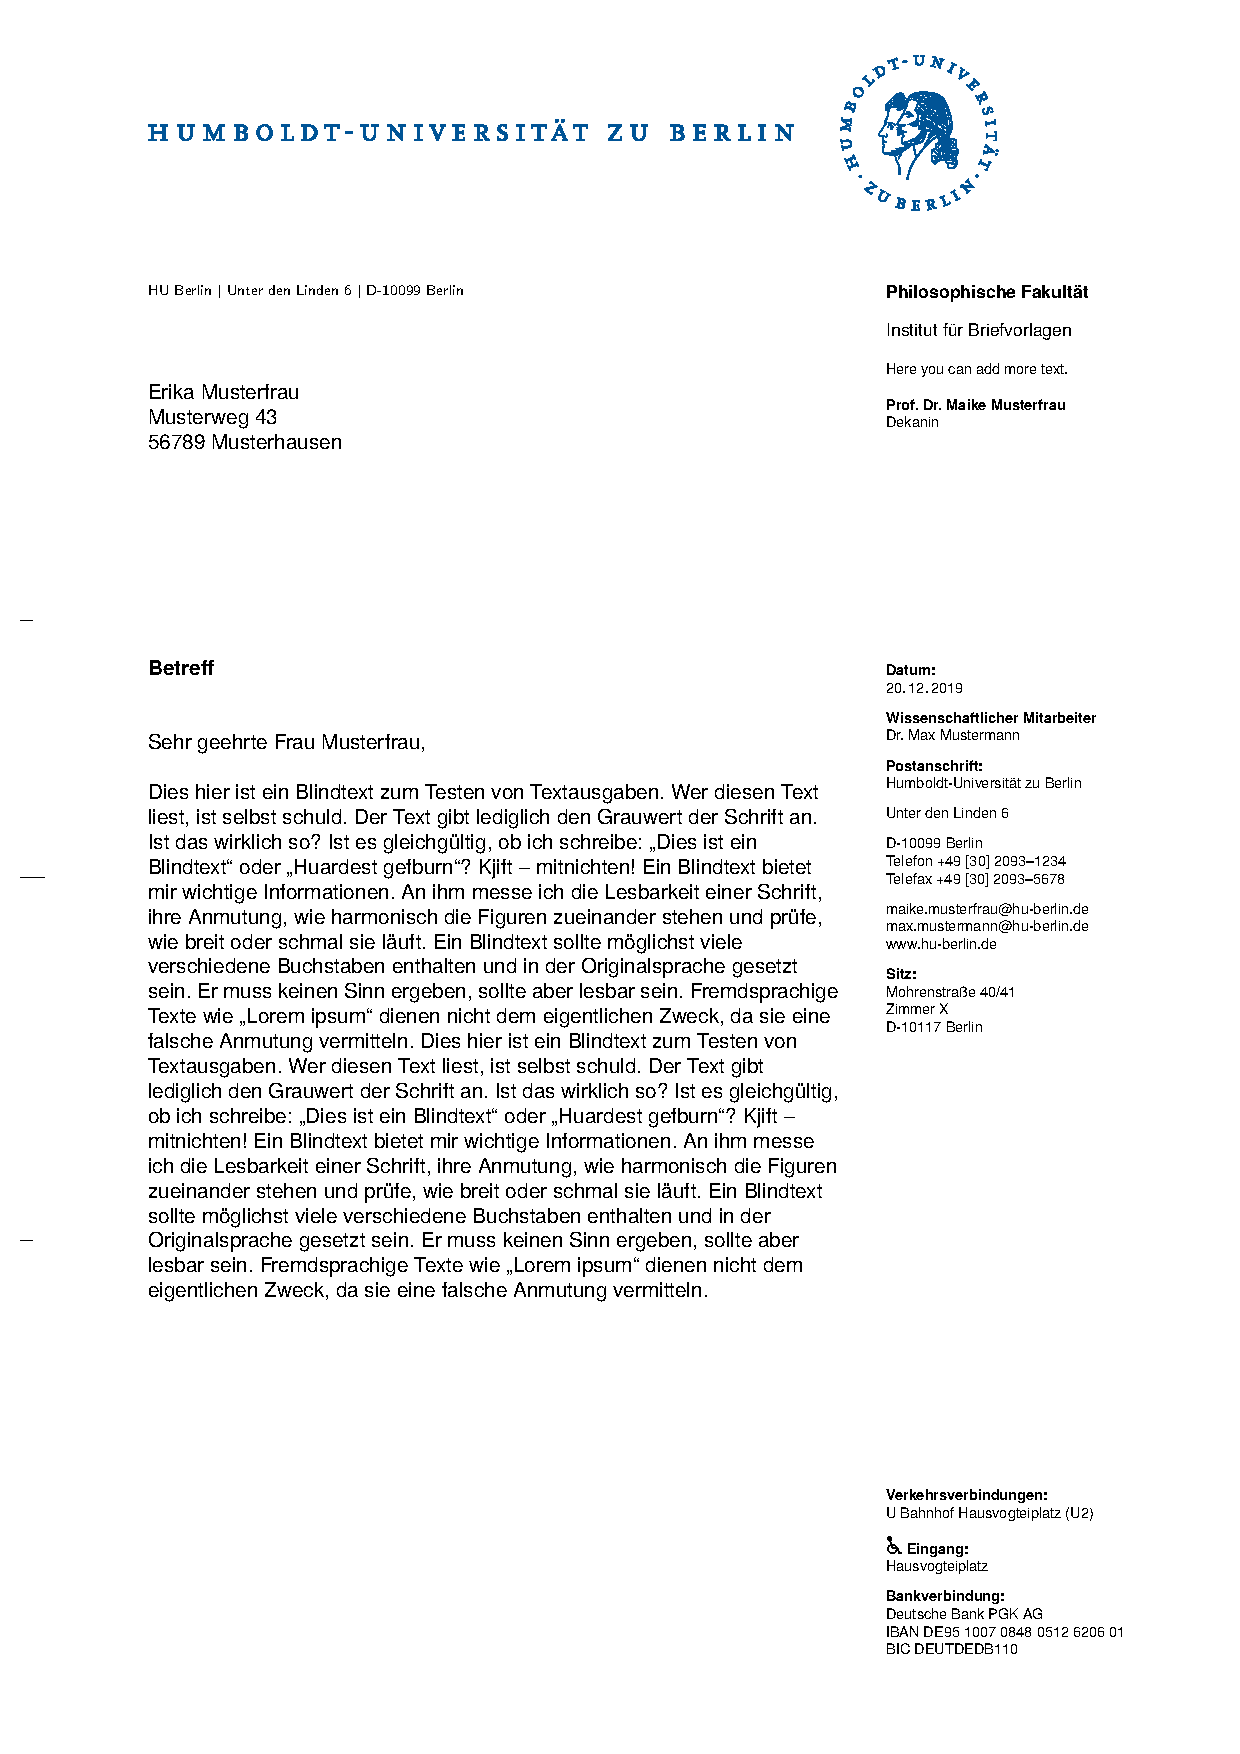
\includepdf[%
  pagecommand={\pagestyle{scrheadings}}
 ,link
 ,pages=-
 % ,scale=.5
 ,nup=2x1
 ,frame]{hu-berlin-letter-example-lualatex.pdf}}
 {|hu-berlin-letter-example-lualatex.pdf| missing!}

\section{From \texttt{.md}}
\IfFileExists{hu-berlin-letter-example-markdown.pdf}
  {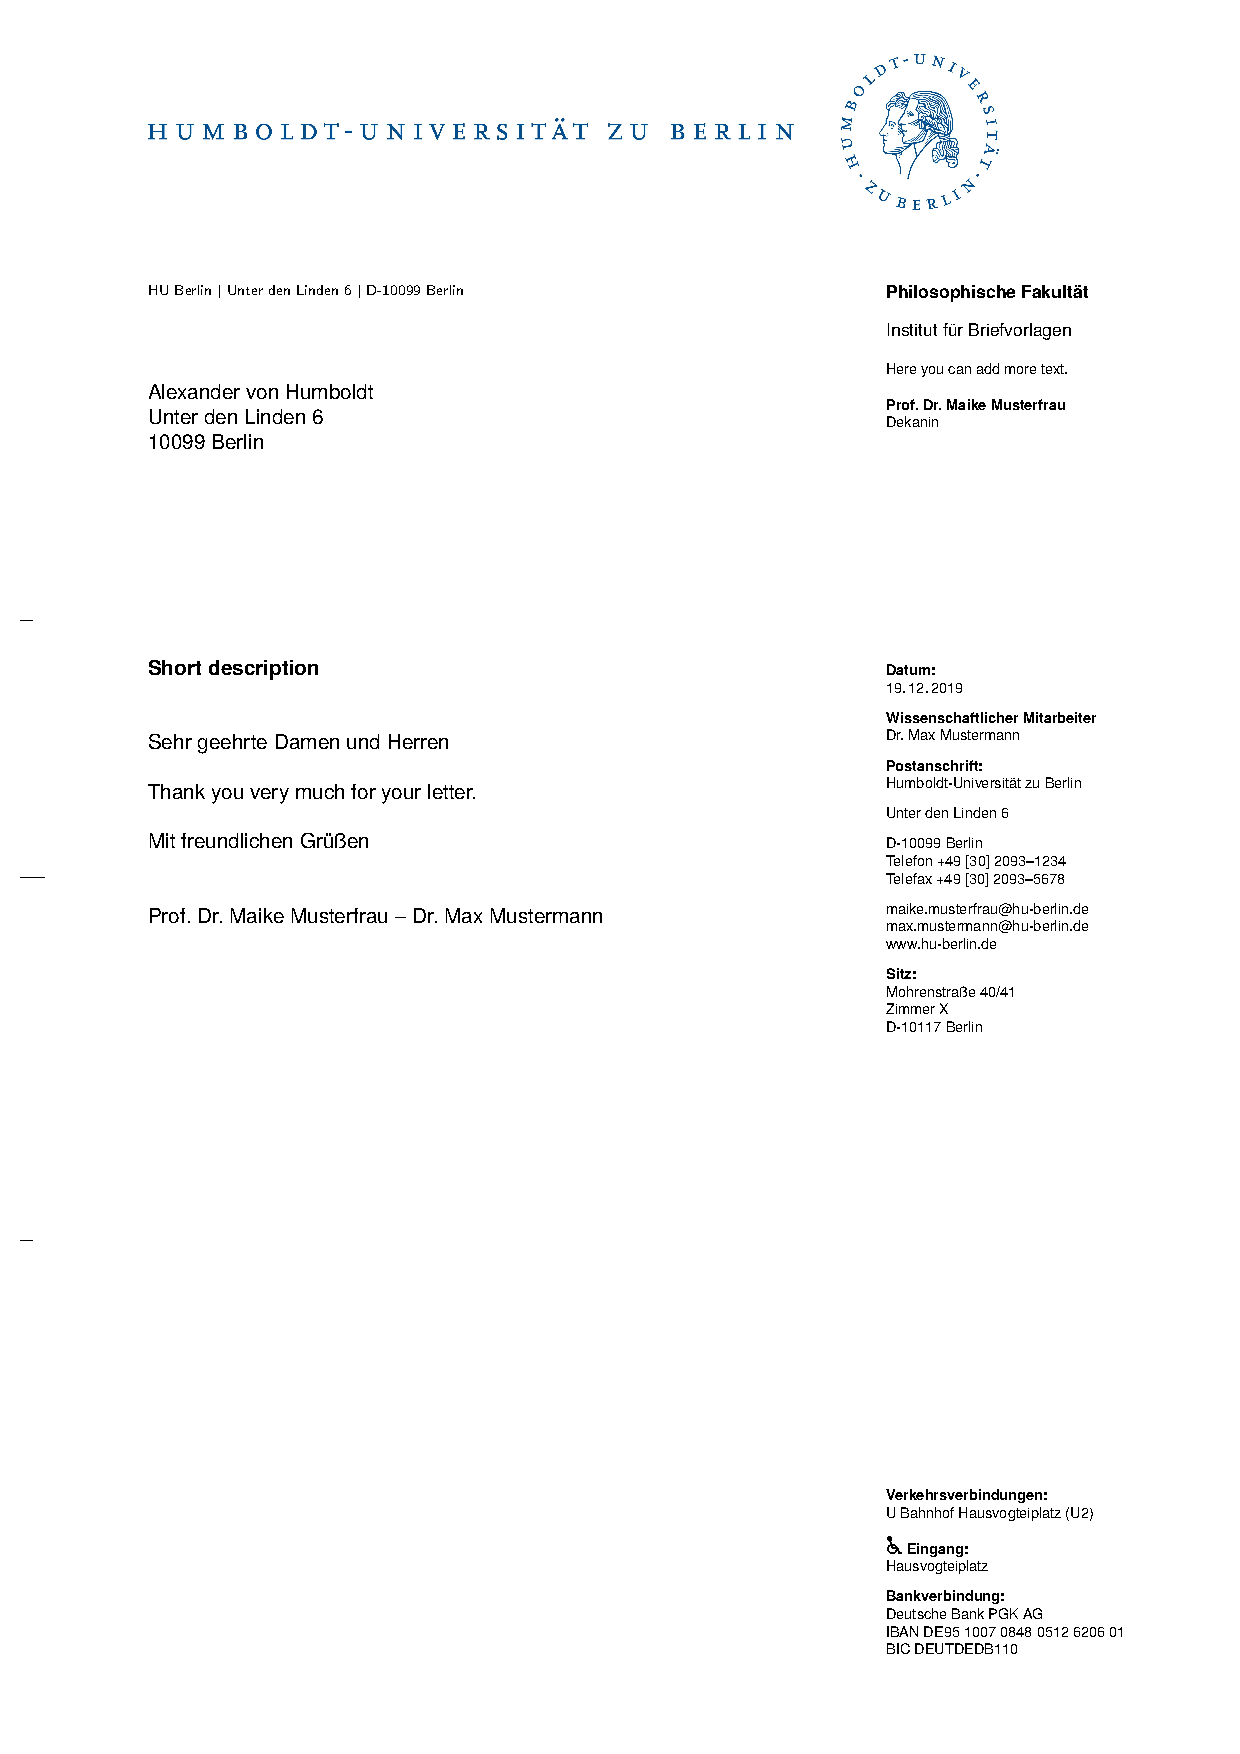
\includepdf[%
  pagecommand={\pagestyle{scrheadings}}
 ,link
 ,pages=-
 % ,scale=.5
 ,nup=2x1
 ,frame]{hu-berlin-letter-example-markdown.pdf}}
 {|hu-berlin-letter-example-markdown.pdf| missing!}


\end{document}
%</driver>
% /*
%     ██ ██████   ██████   ██████ ██    ██ ███    ███ ███████ ███    ██ ████████
%    ██  ██   ██ ██    ██ ██      ██    ██ ████  ████ ██      ████   ██    ██
%   ██   ██   ██ ██    ██ ██      ██    ██ ██ ████ ██ █████   ██ ██  ██    ██
%  ██    ██   ██ ██    ██ ██      ██    ██ ██  ██  ██ ██      ██  ██ ██    ██
% ██     ██████   ██████   ██████  ██████  ██      ██ ███████ ██   ████    ██
% */
% /*
%            ██████  ██████  ██████  ███████
%           ██      ██    ██ ██   ██ ██
% █████     ██      ██    ██ ██   ██ █████       █████
%           ██      ██    ██ ██   ██ ██
%            ██████  ██████  ██████  ███████
% */
% \fi
%
% \part{Guideline for Users} 
%    \begin{macrocode}
%<*example>
%    \end{macrocode}
% \chapter{Letter}
% We give an example on how to create a letter.
%
% \section{\texttt{.lco}-file}
%    \begin{macrocode}
%<*lco>
%    \end{macrocode}
% This is the file you load into your |.tex| letter. 
% The information you provide here do normally not change from letter to letter.
% That’s why we put it in a separate file.
%
% The first line should provide this information.
%    \begin{macrocode}
\ProvidesFile{hu-berlin-letter-example.lco}
%    \end{macrocode}
% Now we set up the personal data.
%
% We start with the name of the sender.
%    \begin{macrocode}
\setkomavar{fromname}
%    \end{macrocode}
% you can also write the position of this person in brackets, this is optional; 
% \oarg{position}
%    \begin{macrocode}
  [Wissenschaftlicher Mitarbeiter]
%    \end{macrocode}
% But you need to give a name:
%    \begin{macrocode}
  {Dr. Max Mustermann} 
%    \end{macrocode}
% The mail address
%    \begin{macrocode}
\setkomavar{fromemail}{max.mustermann@hu-berlin.de}
%    \end{macrocode}
% For phone and fax number you only need to type the last digits.
%    \begin{macrocode}
\setkomavar{fromphone}{1234}
%    \end{macrocode}
% If you don’t have a fax (or a phone),
% leave it empty. Do \emph{not} delete it.
%    \begin{macrocode}
\setkomavar{fromfax}{5678}
%    \end{macrocode}
% And finally the URL.
%    \begin{macrocode}
\setkomavar{fromurl}{www.hu-berlin.de}
%    \end{macrocode}
% If your backaddress is to long 
% – it will be set up automatically – 
% you can redefine it.
% 
%    \begin{macrocode}
%% \setkomavar{backaddress}{HU Berlin\\
%% Unter den Linden 6\\
%% D-10099 Berlin} 
%    \end{macrocode}
% Selfexplaining: the faculty.
%    \begin{macrocode}
\setkomavar{faculty}{%
Philosophische Fakultät
}
%    \end{macrocode}
%
%    \begin{macrocode}
\setkomavar{institute}{%
  \mbox{Institut für Briefvorlagen}
}
%    \end{macrocode}
%    \begin{macrocode}
\setkomavar{institute.additional}{Here you can add more text.}
%    \end{macrocode}
%    \begin{macrocode}
\setkomavar{institute.head}[Dekanin]{Prof. Dr. Maike Musterfrau}
%    \end{macrocode}
%    \begin{macrocode}
\setkomavar{institute.head.mail}{maike.musterfrau@hu-berlin.de}
%    \end{macrocode}
%    \begin{macrocode}
\setkomavar{office}{%
  Mohrenstraße 40/41\\
  Zimmer X\\
  D-10117 Berlin}
%    \end{macrocode}
%    \begin{macrocode}
\setkomavar{connections}{U Bahnhof Hausvogteiplatz (U2)}
%    \end{macrocode}
%    \begin{macrocode}
\setkomavar{accessibility}{Hausvogteiplatz}
%    \end{macrocode}
%    \begin{macrocode}
\setkomavar{signature}{%
  \usekomavar{institute.head} -- 
  \usekomavar{fromname}
}
%    \end{macrocode}
%    \begin{macrocode}
%</lco>
%    \end{macrocode}
% \huberlinlisting%
%  [listing options = {%
%	,linerange={18-48}
%   ,numbers     = left
%   ,numbersep   = 10pt
%   ,numberstyle =\footnotesize\ttfamily\color{hu-berlin-grey}
%   }]%
%  {hu-berlin-letter-example.lco}
%
% \section{\texttt{.tex}-file}
%    \begin{macrocode}
%<*letter>
%    \end{macrocode}
%    \begin{macrocode}
\documentclass{hu-berlin-letter}
%    \end{macrocode}
% Now we load the personal data-file which has the ending |.lco|.
%    \begin{macrocode}
\LoadLetterOption{hu-berlin-letter-example}
%    \end{macrocode}
% If you have the HU font installed on your computer, 
% you can load it, too:
%    \begin{macrocode}
% \setmainfont[%
%   BoldFont=ScalaSans-BoldLF,
%   Numbers=OldStyle]{ScalaSans-RegularLF}
%    \end{macrocode}
% Now following the reference information
%    \begin{macrocode}
\setkomavar{myref}{} 
%    \end{macrocode}
%    \begin{macrocode}
\setkomavar{yourref}{} 
%    \end{macrocode}
%    \begin{macrocode}
\setkomavar{yourmail}{}
%    \end{macrocode}
%    \begin{macrocode}
\setkomavar{customer}{}
%    \end{macrocode}
%    \begin{macrocode}
\setkomavar{invoice}{}
%    \end{macrocode}
%    \begin{macrocode}
\setkomavar{subject}{Betreff}
%    \end{macrocode}
%    \begin{macrocode}
\usepackage{blindtext}
%    \end{macrocode}
% We close the preamble and start the letter
%    \begin{macrocode}
\begin{document}
%    \end{macrocode}
% The address is written as \marg{address} 
%    \begin{macrocode}
\begin{letter}{%
%    \end{macrocode}
%    \begin{macrocode}
  Erika Musterfrau\par
  Musterweg 43\par
  56789 Musterhausen%
%    \end{macrocode}
% Closing now again.
%    \begin{macrocode}
}
%    \end{macrocode}
%    \begin{macrocode}
\opening{Sehr geehrte Frau Musterfrau,}
%    \end{macrocode}
% This is just some blindtext.
%    \begin{macrocode}
\blindtext[2]
\clearpage
\blindtext
%    \end{macrocode}
% Closing letter 
%    \begin{macrocode}
\closing{Mit freundlichen Grüßen}
%    \end{macrocode}
% If you still have something to say/write.
%    \begin{macrocode}
\ps PS: \dots
%    \end{macrocode}
% Any amendment.
%    \begin{macrocode}
\encl{%
  Anlage 1\\
  Anlage 2%
}
%    \end{macrocode}
% This is the distribution
%    \begin{macrocode}
\cc{%
  Verteiler 1\\
  Verteiler 2%
}
%    \end{macrocode}
% That’s it. Done.
%    \begin{macrocode}
\end{letter}
\end{document}
%    \end{macrocode}
% And how does a example letter looks like?
% \huberlinlisting%
%  [listing options = {%
%	,linerange={18-48}
%   ,numbers     = left
%   ,numbersep   = 10pt
%   ,numberstyle =\footnotesize\ttfamily\color{hu-berlin-grey}
%   }]%
%  {hu-berlin-letter-example-lualatex.tex}
%    \begin{macrocode}
%</letter>
%    \end{macrocode}
% \section{Letter from markdown}
%    \begin{macrocode}
%<*letter-md>
%    \end{macrocode}
% You need to have |pandoc| installed on your computer.
% To create letters via markdown and |pandoc| run from the command line:
%
% \begin{warning}pandoc --pdf-engine=lualatex --template hu-berlin-letter-template.latex -o YOUR-FILE.pdf YOUR-FILE.md\end{warning}
% The |.md| file needs a section with metadata.
%
% It starts and ends with three |---|.
% All necessary metadata information are listed inbetween.
%    \begin{macrocode}
---
documentclass: hu-berlin-letter
%    \end{macrocode}
% The following will load the |.lco|-file, you replace that with the name of your |.lco|-file.
%    \begin{macrocode}
sender: hu-berlin-letter-example
%    \end{macrocode}
% You should also tell a short subject
%    \begin{macrocode}
subject: Short description
%    \end{macrocode}
% And if you want to have a different language, define it now. 
% You can choose between German (default)
% and English.
%    \begin{macrocode}
lang: english
%    \end{macrocode}
% The information for the addressee has to be written like this:
%    \begin{macrocode}
addressee:
	- Alexander von Humboldt
	- Unter den Linden 6
	- 10099 Berlin
%    \end{macrocode}
%    \begin{macrocode}
---
%    \end{macrocode}
% You find a list with possible options for this metadata information header below.
%
% Now the content of your letter
%    \begin{macrocode}
Thank you very much for your letter.
%    \end{macrocode}
% Let’s see how this example file looks like:
% \huberlinlisting%
%  [listing options = {%
%   ,numbers     = left
%   ,numbersep   = 10pt
%   ,numberstyle =\footnotesize\ttfamily\color{hu-berlin-grey}
%   }]%
%  {hu-berlin-letter-example-markdown.md}
%    \begin{macrocode}
%</letter-md>
%    \end{macrocode}
% Here we close the example files.
%    \begin{macrocode}
%</example>
%    \end{macrocode}
%\part{Guide for Coders}
%    \begin{macrocode}
%<*sty>
%    \end{macrocode}
%\chapter{hu-berlin-base-package}
%    \begin{macrocode}
%<*base>
%    \end{macrocode}
% Since we do want to compile with \lualatex, 
% we make sure that it will be compilable only with that.
%    \begin{macrocode}
\RequirePackage{ifluatex,luatex85}
%    \end{macrocode}
% Now a fix.\fnurl{https://tex.stackexchange.com/a/75065}
%    \begin{macrocode}
\ifx\directlua\relax
  \let\directlua\UnDeFiNeD
\fi
%    \end{macrocode}
%    \begin{macrocode}
\ifluatex
\else
\GenericError{hu-berlin}%
 {Please use `LuaLaTeX' as Compiler.^^J I abort here.}
\fi
%    \end{macrocode}
% We do not need many packages. 
% The ones we need are loaded now.
%    \begin{macrocode}
\RequirePackage[english,ngerman]{babel}
%    \end{macrocode}
% Common package for handling figures is \pkg{graphicx}.
%    \begin{macrocode}
\RequirePackage{graphicx}
%    \end{macrocode}
% For loading fonts.
%    \begin{macrocode}
\RequirePackage{fontspec}
%    \end{macrocode}
% Actually the corporate design says
% that the font Verdana should be used.
% But since this font is not included in
% UNIX-systems we use a derivative.
%    \begin{macrocode}
\setmainfont{TeX Gyre Heros}
%    \end{macrocode}
% If you have Verdana on your system
% you can uncomment the following line.
%    \begin{macrocode}
% \setmainfont{Verdana}
%    \end{macrocode}
% For the wheelchair symbol we load \pkg{marvosym}
%    \begin{macrocode}
\RequirePackage{marvosym}
%    \end{macrocode}
% And we define various colors from the corporate design manual.
%    \begin{macrocode}
\RequirePackage{xcolor}
\definecolor{hu-berlin-blue}{RGB}{0,65,137}
\definecolor{hu-berlin-green}{RGB}{150,190,20}
\definecolor{hu-berlin-grey}{RGB}{169,169,169}
\definecolor{hu-berlin-brown}{RGB}{82,79,60}
\definecolor{hu-berlin-red}{RGB}{180,0,0}
%    \end{macrocode}
% That’s all for the base package, so we close it.
%    \begin{macrocode}
%</base>
%    \end{macrocode}
%    \begin{macrocode}
%</sty>
%    \end{macrocode}
%    \begin{macrocode}
%<*cls>
%    \end{macrocode}
%\chapter{Letter}
%    \begin{macrocode}
%<*letter>
%    \end{macrocode}
% We load \pkg{scrlttr2} which is the documentclass for letters.
% Furthermore we set up some options.
% The default language is German. But all strings are also 
% available for English. You can load English as option to the 
% documentclass.
%    \begin{macrocode}
\DeclareOption*{\PassOptionsToClass{\CurrentOption}{scrlttr2}}
\DeclareOption{english}{\PassOptionsToPackage{ngerman,main=english}{babel}}
\DeclareOption{ngerman}{\PassOptionsToPackage{ngerman}{babel}}
\ExecuteOptions{ngerman}
\ProcessOptions\relax
%    \end{macrocode}
% Now the documentclass itself.
%    \begin{macrocode}
\LoadClass[%
  fontsize=10pt,
  version=last,
%    \end{macrocode}
% If there is anything to debug, you can enable |visualize|
%    \begin{macrocode}
  % visualize
%    \end{macrocode}
%    \begin{macrocode}
]{scrlttr2}
%    \end{macrocode}
% For debugging also uncomment the \cs{showfields}\marg{fields} commanand.
%    \begin{macrocode}
% \showfields{head,address,location,refline,foot}
%    \end{macrocode}
% Since all common and basic features of the bundle
% are located in a separate package we load that first.
%    \begin{macrocode}
\RequirePackage{hu-berlin-base}
%    \end{macrocode}
% To get the HU logo on the second and following pages we load \pkg{scrlayer-scrpage}.\fnurl{https://tex.stackexchange.com/a/495258/98739}
%    \begin{macrocode}
\RequirePackage{scrlayer-scrpage}
\clearpairofpagestyles
\DeclareNewLayer[
 foreground,
 voffset=\useplength{firstheadvpos},
 hoffset=\useplength{firstheadhpos},
 width=\useplength{firstheadwidth},
 mode=picture,
 contents=\putUL{\raisebox{-\height}{\usekomavar{firsthead}}}
]{likefirstpage.head}
\AddLayersToPageStyle{scrheadings}{likefirstpage.head}
\DeclareNewLayer[
 foreground,
 align=r,
 voffset=\useplength{locvpos},
 hoffset=\paperwidth-\useplength{lochpos},
 width=\useplength{locwidth},
 height=\useplength{locheight},
 contents=\usekomavar{nextlocation},
 %pretocontents=\layercontentsmeasure% to show the position of the layer
]{likefirstpage.loc}
\AddLayersToPageStyle{scrheadings}{likefirstpage.head,likefirstpage.loc}
%    \end{macrocode}
% Now we apply the code for following pages.
%    \begin{macrocode}
\newkomavar{nextlocation}
\setkomavar{nextlocation}{%
  \raggedright
  \fontsize{7}{8.5}\selectfont
  \pagemark
}
%    \end{macrocode}
% For better adjustments of the layout we load \pkg{geometry}.
%    \begin{macrocode}
\RequirePackage{geometry}
\geometry{%
  a4paper
 ,left           =25mm
 ,bottom         =16mm
 ,foot           =4mm
 ,top            =77mm
 ,headheight     =15pt
 ,textwidth      =117mm
 ,marginparsep   =0mm
 ,marginparwidth =0mm
}
%    \end{macrocode}
% Main Text and signature should be raggedright.
%    \begin{macrocode}
\renewcommand*{\raggedsignature}{\raggedright}
\raggedright
%    \end{macrocode}
% We also want to put the enclosures at the bottom of the page.\fnurl{https://tex.stackexchange.com/questions/77991/put-the-encl-at-the-bottom-of-the-page-lettre-class}
%    \begin{macrocode}
\def\stopletter{}
\let\enclold\encl 
\renewcommand\encl[1]{\vskip0ptplus1filll\enclold{#1}}
%    \end{macrocode}
% We define new |komavar|s and we make it for 
% German and for English as well.
%    \begin{macrocode}
\providecaptionname{english}{\hubCCseparator}{Copy to}
\providecaptionname{english}{\hubEnclSeparator}{Attachment}
\providecaptionname{english}{\hubMyRef}{Reference:}
\providecaptionname{english}{\hubFromName}{Clerk:}
\providecaptionname{english}{\hubDate}{Date:}
\providecaptionname{english}{\hubAddress}{Postal address:}
\providecaptionname{english}{\hubConnections}{Public transport:}
\providecaptionname{english}{\hubOffice}{Office:}
\providecaptionname{english}{\hubBank}{Bank:}
\providecaptionname{english}{\hubOfficeHours}{Consultation hours:}
\providecaptionname{english}{\hubAccessibility}{Entrance:}
%    \end{macrocode}
% Now for German.
%    \begin{macrocode}
\providecaptionname{ngerman}{\hubCCseparator}{Kopie an}
\providecaptionname{ngerman}{\hubEnclSeparator}{Anlage}
\providecaptionname{ngerman}{\hubMyRef}{Geschäftszeichen:}
\providecaptionname{ngerman}{\hubFromName}{Bearbeiter:}
\providecaptionname{ngerman}{\hubDate}{Datum:}
\providecaptionname{ngerman}{\hubAddress}{Postanschrift:}
\providecaptionname{ngerman}{\hubConnections}{Verkehrsverbindungen:}
\providecaptionname{ngerman}{\hubOffice}{Sitz:}
\providecaptionname{ngerman}{\hubBank}{Bank:}
\providecaptionname{ngerman}{\hubOfficeHours}{Sprechzeiten:}
\providecaptionname{ngerman}{\hubAccessibility}{Eingang:}
%    \end{macrocode}
% First the possibility to name the faculty,
%    \begin{macrocode}
\newkomavar{faculty}
\newkomafont{faculty}{\bfseries\fontsize{8.5}{10}\selectfont}
%    \end{macrocode}
% then the institute
%    \begin{macrocode}
\newkomavar{institute}
\newkomafont{institute}{\fontsize{8.5}{10}\selectfont}
%    \end{macrocode}
% and further fields for information.
%    \begin{macrocode}
\newkomavar{institute.additional}
%    \end{macrocode}
% We pass the name of the head of the institute.
%    \begin{macrocode}
\newkomafont{institute.head}{\bfseries}
\newkomavar{institute.head}%
%    \end{macrocode}
% Its position will be written as the optional argument.
%
% There is even the possibility to print the email-address onto the letter.
%    \begin{macrocode}
\newkomavar{institute.head.mail}%
%    \end{macrocode}
% Since there are many buildings with offices we tell where to find the sender
%    \begin{macrocode}
\newkomavar{office}
\setkomavar*{office}{\hubOffice}
%    \end{macrocode}
% and how to get there.
%    \begin{macrocode}
\newkomavar{connections}
\setkomavar*{connections}{\hubConnections}
%    \end{macrocode}
% Furthermore we inform about office hours
%    \begin{macrocode}
\newkomavar{officehours}
\setkomavar*{officehours}{\hubOfficeHours}
%    \end{macrocode}
% and if there is accessibility for wheelchairs etc.
%    \begin{macrocode}
\newkomavar{accessibility}
\setkomavar*{accessibility}{{\large\reflectbox{\Wheelchair}} \hubAccessibility}
%    \end{macrocode}
%    \begin{macrocode}
\newkomavar{bank}
\setkomavar*{bank}{\hubBank}
\setkomavar{bank}{Deutsche Bank PGK AG}
\newkomavar{IBAN}
\setkomavar{IBAN}{\mbox{IBAN DE95 1007 0848 0512 6206 01}}
\newkomavar{BIC}
\setkomavar{BIC}{BIC DEUTDEDB110}
%    \end{macrocode}
% Now we set the location field,
% which is the section on the right with additional information:
%    \begin{macrocode}
\setkomavar{location}{%
%    \end{macrocode}
% First anything regarding the font
%    \begin{macrocode}
  \raggedright
  \fontsize{7}{8.5}\selectfont
%    \begin{macrocode}
% and for the section of faculty, institute etc. we use \env{minipage}
%    \begin{macrocode}
\begin{minipage}[t][64mm]{\useplength{locwidth}}
%    \end{macrocode}
% then the faculty
%    \begin{macrocode}
\Ifkomavarempty{faculty}
%    \end{macrocode}
% This is a fake space to avoid any trouble 
% if no custom metadata are given.
%    \begin{macrocode}
  {\hspace*{1em}}
  {\usekomafont{faculty}%
   \usekomavar{faculty}\\[1\baselineskip]}
%    \end{macrocode}
% and the institute.
%    \begin{macrocode}
\Ifkomavarempty{institute}
  {}
  {\usekomafont{institute}\usekomavar{institute}\\[1\baselineskip]}
%    \end{macrocode}
% Now anything else regarding the institute.
%    \begin{macrocode}
\Ifkomavarempty{institute.additional}
  {}
  {\usekomavar{institute.additional}\\[1\baselineskip]}
%    \end{macrocode}
% What follows is the head of institute and its position name.
%    \begin{macrocode}
\Ifkomavarempty{institute.head}
 {}
 {{\usekomafont{institute.head}%
  \usekomavar{institute.head}}\\%
 \usekomavar*{institute.head}}
%    \end{macrocode}
% We close this section and the minipage.
%    \begin{macrocode}
 \end{minipage}
%    \end{macrocode}
% Let’s turn to further information.
%
% For example date:
%    \begin{macrocode}
  \textbf{\usekomavar*{date}}\\
  \usekomavar{date}\par
%    \end{macrocode}
% and the sender of the letter.
%    \begin{macrocode}
\Ifkomavarempty{fromname}
 {}
 {\textbf{\usekomavar*{fromname}}\\
  \usekomavar{fromname}\par}
%    \end{macrocode}
% And the reference of correspondence.
%    \begin{macrocode}
\Ifkomavarempty{myref}
 {}
 {\textbf{\usekomavar*{myref}}\\
  \usekomavar{myref}\par}
%    \end{macrocode}
% To complete this template we provide the possibility to name further reference fields.
%    \begin{macrocode}
\Ifkomavarempty{yourref}
 {}
 {\textbf{\usekomavar*{yourref}}\\
  \usekomavar{yourref}\par}
%    \end{macrocode}
%    \begin{macrocode}
\Ifkomavarempty{yourmail}
 {}
 {\textbf{\usekomavar*{yourmail}}\\
  \usekomavar{yourmail}\par}
%    \end{macrocode}
%    \begin{macrocode}
\Ifkomavarempty{customer}
 {}
 {\textbf{\usekomavar*{customer}}\\
  \usekomavar{customer}\par}
%    \end{macrocode}
%    \begin{macrocode}
\Ifkomavarempty{invoice}
 {}
 {\textbf{\usekomavar*{invoice}}\\
  \usekomavar{invoice}\par}
%    \end{macrocode}
%    \begin{macrocode}
  \textbf{\usekomavar*{fromaddress}}\\
  \usekomavar{fromaddress}
  \Ifkomavarempty{fromphone}
    {\par}
    {\\\usekomavar*{fromphone}\usekomavar{fromphone}
     \Ifkomavarempty{fromfax}
    {\par}
    {\\}}
  \Ifkomavarempty{fromfax}
    {}
    {\usekomavar*{fromfax}\usekomavar{fromfax}\par}
%    \end{macrocode}
% Next, emails and url:
%    \begin{macrocode}
\Ifkomavarempty{institute.head.mail}
  {}
  {\usekomavar{institute.head.mail}
  \Ifkomavarempty{fromemail}
  {\Ifkomavarempty{fromurl}
   {\par}
   {\\}}
  {\\}}
%    \end{macrocode}
%
%    \begin{macrocode}
\Ifkomavarempty{fromemail}
  {}
  {\usekomavar{fromemail}
  \Ifkomavarempty{fromurl}
  {\par}
  {\\}}
%    \end{macrocode}
%
%    \begin{macrocode}
\Ifkomavarempty{fromurl}
  {}
  {\usekomavar{fromurl}\par}
%    \end{macrocode}
% Now the actual location of the sender
%    \begin{macrocode}
\Ifkomavarempty{office}
  {}
  {\textbf{\usekomavar*{office}}\\
  \usekomavar{office}\par}
%    \end{macrocode}
% The last information section should be pinned to the bottom.
%    \begin{macrocode}
\vfill
%    \end{macrocode}
% Inform your addressee about the connection possibilities.
%    \begin{macrocode}
\Ifkomavarempty{connections}
  {}
  {\textbf{\usekomavar*{connections}}\\
  \usekomavar{connections}\par}
%    \end{macrocode}
%    \begin{macrocode}
\Ifkomavarempty{officehours}
  {}
  {\textbf{\usekomavar*{officehours}}\\
  \usekomavar{officehours}\par}
%    \end{macrocode}
% If there is a barrier free entrance, tell it.
%    \begin{macrocode}
\Ifkomavarempty{accessibility}
  {}
  {\textbf{\usekomavar*{accessibility}}\\
  \usekomavar{accessibility}\par}
%    \end{macrocode}
% And last the bank connection
%    \begin{macrocode}
\Ifkomavarempty{bank}
  {}
  {\textbf{\usekomavar*{bank}}\\
  \usekomavar{bank}\\
  \usekomavar{IBAN}\\
  \usekomavar{BIC}
  }
%    \end{macrocode}
% Finally we close \cs{setkomavar}\marg{location}
%    \begin{macrocode}
}
%    \end{macrocode}
% To fulfill the Corporate Design rules we adjust a few things.
%    \begin{macrocode}
\KOMAoptions{%
   numericaldate =true
  ,refline       =nodate
  ,backaddress   =plain
  ,parskip       =half-
}
%    \end{macrocode}
% Getting rid of all other fields and their default position.
%    \begin{macrocode}
\removereffields
%    \end{macrocode}
% Redefining length.
%    \begin{macrocode}
\setplength{refvpos}{110mm}
\setplength{refaftervskip}{0pt}
\setplength{toaddrhpos}{25mm}
\setplength{firstheadhpos}{\useplength{toaddrhpos}}
\setplength{lochpos}{15mm}
\setplength{locvpos}{\useplength{toaddrvpos}}
\addtoplength{locvpos}{.75\baselineskip}
\setplength{locwidth}{45mm}
\setplength{locheight}{232mm}
%    \end{macrocode}
% Now resetting or pre-defining some variables.
%
% First we set the head of the first page,
% which is the logo. 
% Be sure that you have the right using it!
% Everything regarding the logo is defined in
% the corporate design guidlines.\fnurl{https://www.hu-berlin.de/de/hu-intern/design/basiselemente/leitfaden-corporate-design-hu.pdf}
% You need to have the actual logo of the Humboldt-Universität zu Berlin which has to be called |hu-berlin-logo.pdf|.
% It can be downloaded here: \url{http://zope.hu-berlin.de/hu-intern/design/downloads/logo}
% If this logo is not found a replacement text is shown instead.
%    \begin{macrocode}
\setkomavar{firsthead}{%
\IfFileExists{hu-berlin-logo.pdf}
  {
\includegraphics[width=145mm]{hu-berlin-logo.pdf}}
  {{\vspace*{2em}\hfil\scshape [humboldt-universität zu berlin]}}%
}
%    \end{macrocode}
%
%    \begin{macrocode}
\setkomavar{backaddressseparator}{~\textbar~}
%    \end{macrocode}
%
%    \begin{macrocode}
\setkomavar{fromphone}{0000}
\setkomavar*{fromphone}{Telefon +49 [30] 2093–}
%    \end{macrocode}
%
%    \begin{macrocode}
\setkomavar{fromfax}{0000}
\setkomavar*{fromfax}{Telefax +49 [30] 2093–}
%    \end{macrocode}
%
%    \begin{macrocode}
\setkomavar*{fromaddress}{\hubAddress}
\setkomavar{fromaddress}{%
  Humboldt-Universität zu Berlin\\
  Unter den Linden 6\\
  D-10099 Berlin}
%    \end{macrocode}
% The default backaddress is slightly changed:
%    \begin{macrocode}
\setkomavar{backaddress}{%
  Humboldt-Universität zu Berlin\\
  UdL 6\\
  D-10099 Berlin}
%    \end{macrocode}
%
%    \begin{macrocode}
\setkomavar*{date}{\hubDate}
%    \end{macrocode}
%
%    \begin{macrocode}
\setkomavar*{fromname}{\hubFromName}
%    \end{macrocode}
%
%    \begin{macrocode}
\setkomavar*{myref}{\hubMyRef}
%    \end{macrocode}
%    \begin{macrocode}
\setkomavar*{enclseparator}{\hubEnclSeparator}
%    \end{macrocode}
%    \begin{macrocode}
\setkomavar*{ccseparator}{\hubCCseparator} 
%    \end{macrocode}
%    \begin{macrocode}
% \RequirePackage{hyperref}
% \AtBeginDocument{{
%   \usekomavar[\def\author]{fromname}
%   \usekomavar[\def\subject]{subject}
%   \hypersetup{%
%     pdftitle           = {\subject},
%     pdfauthor          = {\author},
%     pdfsubject         = {\subject},
%     pdfkeywords        = {\author, \subject},
%     pdflang            = de,
%     pdfdisplaydoctitle = true,
%     colorlinks         = true,
%     plainpages         = false,
%     hypertexnames      = false,
%     unicode,
%   }
% }}
%    \end{macrocode}
%    \begin{macrocode}
%</letter>
%    \end{macrocode}
%    \begin{macrocode}
%</cls>
%    \end{macrocode}
%    \begin{macrocode}
%<*template>
%    \end{macrocode}
% \chapter{Boilerplate / Template for letters }
%    \begin{macrocode}
%<*letter-md>
%    \end{macrocode}
% Defining the documentclass and the language, too.
%    \begin{macrocode}
\documentclass[
$if(lang)$$lang$$else$german$endif$
]{hu-berlin-letter}
%    \end{macrocode}
% We predefine two  variables.
%    \begin{macrocode}
\newkomavar{opening}
\newkomavar{closing}
\setkomavar{opening}{Sehr geehrte Damen und Herren}
\setkomavar{closing}{Mit freundlichen Grüßen}
%    \end{macrocode}
%    \begin{macrocode}
$for(letteroption)$
\LoadLetterOption{$letteroption$}
$endfor$
$if(sender)$\LoadLetterOption{$sender$}$endif$
$if(addresseeimage)$\setkomavar{addresseeimage}{$addresseeimage$}$endif$
$if(backaddress)$\setkomavar{backaddress}{$backaddress$}\KOMAoptions{backaddress=true}$endif$
$if(fromalign)$\KOMAoptions{fromalign=$fromalign$}$endif$
$if(customer)$\setkomavar{customer}{$customer$}$endif$
$if(date)$\setkomavar{date}{$date$}$endif$
$if(fromaddress)$\setkomavar{fromaddress}{$fromaddress$}$endif$
$if(frombank)$\setkomavar{frombank}{$frombank$}$endif$
$if(fromemail)$\setkomavar{fromemail}{$fromemail$}\KOMAoptions{fromemail=true}$endif$
$if(fromfax)$\setkomavar{fromfax}{$fromfax$}\KOMAoptions{fromfax=true}$endif$
$if(fromlogo)$\setkomavar{fromlogo}{$fromlogo$}\KOMAoptions{fromlogo=true}$endif$
$if(frommobilephone)$\setkomavar{frommobilephone}{$frommobilephone$}\KOMAoptions{frommobilephone=true}$endif$
$if(fromname)$\setkomavar{fromname}{$fromname$}$endif$
$if(fromphone)$\setkomavar{fromphone}{$fromphone$}\KOMAoptions{fromphone=true}$endif$
$if(fromurl)$\setkomavar{fromurl}{$fromurl$}\KOMAoptions{fromurl=true}$endif$
$if(fromzipcode)$\setkomavar{fromzipcode}{$fromzipcode$}$endif$
$if(invoice)$\setkomavar{invoice}{$invoice$}$endif$
$if(location)$\setkomavar{location}{$location$}$endif$
$if(myref)$\setkomavar{myref}{$myref$}$endif$
$if(myrefname)$\setkomavar*{myref}{$myrefname$}$endif$
$if(place)$\setkomavar{place}{$place$}$endif$
$if(PPcode)$\setkomavar{PPcode}{$PPcode$}$endif$
$if(signature)$\setkomavar{signature}{$signature$}$endif$
$if(specialmail)$\setkomavar{specialmail}{$specialmail$}$endif$
$if(subject)$\setkomavar{subject}{$subject$}$endif$
$if(title)$\setkomavar{title}{$title$}$endif$
$if(yourmail)$\setkomavar{yourmail}{$yourmail$}$endif$
$if(yourref)$\setkomavar{yourref}{$yourref$}$endif$
$if(opening)$\setkomavar{opening}{$opening$}$endif$
$if(closing)$\setkomavar{closing}{$closing$}$endif$
$if(firstfoot)$\setkomavar{firstfoot}{$firstfoot$}$endif$
%    \end{macrocode}
% Ok, let’s sum up the possible options you can use to pass data to the letter:
% \begin{itemize} \item addresseeimage \item backaddress \item customer \item date \item fromaddress \item frombank \item fromemail \item fromfax \item fromlogo \item frommobilephone \item fromname \item fromphone \item fromurl \item fromzipcode \item invoice \item location \item myref \item myrefname \item place \item PPcode \item signature \item specialmail \item subject \item title \item yourmail \item yourref \item opening \item closing \item firstfoot \end{itemize}
% Sometimes you might not have an addressee – we are checking this, too.
%    \begin{macrocode}
$if(addressee)$
$else$
\KOMAoptions{addrfield=false}
$endif$
%    \end{macrocode}
% Now the actual content of the letter
%    \begin{macrocode}
\begin{document}
\begin{letter}{%
$for(addressee)$
$addressee$$sep$\\
$endfor$
}
$for(include-before)$
$include-before$
$endfor$
\opening{\usekomavar{opening}}
$body$
\closing{\usekomavar{closing}}
$if(ps)$\ps{$ps$}$endif$
$if(encl)$\encl{$encl$}$endif$
$for(include-after)$$include-after$$endfor$
\end{letter}
\end{document}
%    \end{macrocode}
%    \begin{macrocode}
%</letter-md>
%</template>
%    \end{macrocode}
%\chapter{Documentation preamble \param{style}}
%    \begin{macrocode}
%<*sty>
%<*style>
\makeatletter
\addtolength\marginparwidth{-40pt}
\addtolength\marginparsep{4mm} 
\addtolength\oddsidemargin{-20pt}
\addtolength\evensidemargin{-20pt}
\let\PrintDescribeMacro=\@gobble
\let\PrintDescribeEnv=\@gobble
% \def\Describe@Macro#1{\endgroup
%     %\marginnote{\PrintDescribeMacro{#1}}%
%     \SpecialUsageIndex{#1}\@esphack\ignorespaces%
%     }
%\def\Describe@Env#1{\endgroup
%     %\marginnote{\PrintDescribeEnv{#1}}%
%     \SpecialEnvIndex{#1}\@esphack\ignorespaces%
%     }
\makeatother
\AtBeginDocument{\normalmarginpar}
\setlength\MacrocodeTopsep{.5\baselineskip}
\setlength\MacroIndent{6mm}


\RequirePackage{luatexbase}
\RequirePackage[ngerman,english]{babel}
\RequirePackage{calc} 

\RequirePackage[
  paper      = a4paper,  %  - use A4 paper size
  foot       = 2cm,
  inner      = 3cm,  %  - total body: left margin (odd pages)
  top        = 3cm,  %  - total body: top margin
  outer      = 3cm,  %  - total body: right margin (odd pages)
  bottom     = 3cm,  %  - total body: bottom margin
  marginparwidth = 2cm,  %  - width for side note
  marginparsep   = .5cm,  %  - space between notes and body text (content)
%  showframe,
]{geometry}

\newlength\fullwidth
\setlength\fullwidth{\textwidth+\marginparwidth+\marginparsep}

\KOMAoptions{
	numbers    = noenddot,
}
\AtBeginDocument{
  \KOMAoptions{
	% headwidth  = {\fullwidth},
	% footwidth  = {\fullwidth},
	footheight = 20pt,
	headheight = 29pt,
	captions   = tableheading,
}}



\title{\huberlintitle}
%\subtitle{\huberlinsubtitle}
\author{\huberlinauthor}
\date{\Version}


%---- Required Packages
\RequirePackage{ifluatex,luatex85}
\ifx\directlua\relax
  \let\directlua\UnDeFiNeD
\fi
\ifluatex
\else
\GenericError{hu-berlin}%
 {Please use `LuaLaTeX' as Compiler.^^J I abort here.}
\fi
%    \end{macrocode}
% For fonts we load the package \pkg{fontspec} which
% has almost no limits handling font-stuff.
%    \begin{macrocode}
\RequirePackage{fontspec}
%    \end{macrocode}
%    \begin{macrocode}
\RequirePackage[mono=false]{libertine}
\RequirePackage{amssymb}

\defaultfontfeatures{%
  Ligatures = TeX
}
%    \end{macrocode}
% For fonts we use the available |TeX Gyre Pagella| as main font.\fnurl{http://www.gust.org.pl/projects/e-foundry/tex-gyre}
%    \begin{macrocode}
\setmainfont[%
   Ligatures = TeX
  ,Numbers   = OldStyle]{TeX Gyre Pagella}
%    \end{macrocode}
% And we declare also the other fonts, too.
%    \begin{macrocode}
\setmonofont[%
  Scale=1
]{TeX Gyre Cursor}
\setsansfont[%
  ,LetterSpace = .8
]{TeX Gyre Adventor-Regular}
\linespread{1.05}
%    \end{macrocode}
%    \begin{macrocode}



\RequirePackage{marginnote}
\renewcommand*{\marginfont}{%
  \rule{0pt}{0.7\baselineskip}%
  \footnotesize%
  \color{hu-berlin-brown}}

\RequirePackage[
  german = guillemets,
  style  = german,
]{csquotes}

\RequirePackage{enumitem}
\setlist{
  nosep, 
  % itemindent=1em,
  % labelindent=0.5\parindent,
  leftmargin=*}
\newlist{tabitemize}{itemize}{2}% neue Listenumgebung 
\setlist[tabitemize]{%
  nosep, 
  leftmargin=*
 } 
\setlist[tabitemize,1]{label=\labelitemi} 
\setlist[tabitemize,2]{label=\labelitemii} 


\clubpenalty=10000  % prevent single lines at the beginning of a paragraph (Schusterjungen)
\widowpenalty=10000  % prevent single lines at the end of a paragraph (Hurenkinder)
\displaywidowpenalty=10000    %

\RequirePackage{pdfpages}
\RequirePackage{biblatex}
\addbibresource{\jobname-bibliography.bib}
\addbibresource{\jobname-ctan.bib}
\RequirePackage{ccicons} %creative commons
\RequirePackage{xparse}
\RequirePackage{ragged2e}
\RequirePackage{microtype}
\RequirePackage{xspace}
\RequirePackage{graphicx}
\graphicspath{{img/}}
%    \end{macrocode}
%    \begin{macrocode}
\RequirePackage{etoolbox}
%https://tex.stackexchange.com/a/235881/98739
\AfterEndPreamble{%
  \maketitle
  \renewcommand\MacroFont{\ttfamily}
  \renewcommand\AltMacroFont{\ttfamily\linespread{.8}}% slanted verbatim
}

% https://tex.stackexchange.com/a/401466/98739
\makeatletter
\renewcommand*{\maketitle}{%
  % taken and shortened from /usr/share/texmf/tex/latex/koma-script/scrartcl.cls
  \begin{titlepage}
  \newgeometry{left=3cm,right=3cm,top=1.5cm,bottom=2cm}
  \global\@topnum=\z@
  \setparsizes{\z@}{\z@}{\z@\@plus 1fil}\par@updaterelative
  \null
   {\large\@author\hfill \href{mailto:lukas@texografie.de}{lukas@texografie.de}\par}
  \vskip 10em%
	{\begin{center}\color{hu-berlin-blue}
	{\fontsize{50}{55}\selectfont\huberlinshort{} \par\vskip .5em%
	\Large\sffamily\@title}\par
	\vskip .5em
	\end{center}}%
	{\ifx\@subtitle\@empty\else\usekomafont{subtitle}\@subtitle\par\fi}%
	\null\vskip 5em%
	\blockcquote[195]{Hoare1973}{Documentation must be regarded as an integral part of the process of design and coding.
 A good programming language will encourage and assist the programmer to write clear,
 self-documenting code,
 and even perhaps to develop
 and display a pleasant style
 of writing.}
	\null\vfill
	{\usekomafont{subtitle}{\@date \hfill
	
\includegraphics[width=4cm]{img/texografie-logo.pdf}\\}}%
  \par
 \vskip 0em
  \restoregeometry
  \end{titlepage}
}%
\makeatother

\RequirePackage{xcolor}
\definecolor{hu-berlin-blue}{RGB}{0,65,137} % HEX 004189
\definecolor{hu-berlin-green}{RGB}{150,190,20} % HEX 93C11A % Topoi
\definecolor{hu-berlin-grey}{RGB}{169,169,169}
\definecolor{hu-berlin-brown}{RGB}{82,79,60}
\definecolor{hu-berlin-red}{RGB}{180,0,0}


\RequirePackage{dirtree}
\renewcommand*\DTstylecomment{%
  \color{hu-berlin-grey}%
  \footnotesize%
  \sffamily}
\renewcommand*\DTstyle{%
  \ttfamily%
  \small%
  }

\RequirePackage[ 
  markcase    = noupper,
  footsepline = .5pt,
  % headsepline = .5pt,
  autooneside = false,% use left and right marks with a onesided document
  automark,% set \leftmark and \rightmark automatically by *\section and \subsection
  draft  = false,
  ]{scrlayer-scrpage} 

\pagestyle{scrheadings}
\clearpairofpagestyles
\rofoot*{\thepage}
\lofoot*{\textcolor{hu-berlin-blue}{\huberlintitle}\ \vrule\ \textcolor{hu-berlin-brown}{\huberlinsubtitle}}
\rohead*{hu-berlin-bundle}
\lohead*{Version: \Version}
%    \end{macrocode}
%    \begin{macrocode}
% https://tex.stackexchange.com/a/352925/98739
\newcommand*\partnumber{}
\DeclareNewLayer[
  background,
  textarea,
  addwidth=\marginparsep+\marginparwidth,
  mode=picture,
  contents={%
	\putC{\makebox[0pt][c]{\raisebox{-.5\height}{\scalebox{50}{\textcolor{black!5}{\partnumber}}}}}\gdef\partnumber{}%
  }
]{partnumber}
\DeclareNewPageStyleByLayers{part}{partnumber}
\renewcommand\partpagestyle{part}
\renewcommand*{\partformat}{\gdef\partnumber{\thepart}}

% only a dirty workaround for the part title
\newcommand*\changedpartwidth[1]{%
  \makebox[\linewidth][l]{%
	\parbox{\dimexpr\textwidth+\marginparsep+\marginparwidth\relax}{\raggedpart#1}%
  }%
}
% add \changedpartwidth as last command to the settings for font element part
\addtokomafont{part}{\Huge\changedpartwidth}



%-https://tex.stackexchange.com/a/339516/98739 | https://tex.stackexchange.com/a/96722/98739
% footnotes in the footer:
\deffootnote%
  %[\normalparindent]%<width of mark>
  {0.0cm}%<indent of footnote text>
  {\normalparindent}%<paragraph indent in the footnote text>
  {\makebox[\normalparindent][r]%
  {\thefootnotemark\hspace*{3pt}}}%<definition of mark>
\newlength{\normalparindent}
\AtBeginDocument{\setlength{\normalparindent}{\parindent}}
 \setfootnoterule{0pt}% Kein Fußnotenstrich
 %\setfootnoterule[<height>]{<length>}

%    \end{macrocode}
% This will put the numbers of the chapters and sections into the margin.
%    \begin{macrocode}
\renewcommand\sectionlinesformat[4]{%
  \makebox[0pt][r]{#3}#4%
}
%    \end{macrocode}
%    \begin{macrocode}
\RequirePackage{url}
%  \urlstyle{same}

\setkomafont{title}{\sffamily\color{hu-berlin-blue}\flushleft\bfseries}
\setkomafont{disposition}{\color{hu-berlin-brown}\sffamily\bfseries\large}
\setkomafont{section}{\usekomafont{disposition}}
\setkomafont{subsection}{\usekomafont{disposition}}
\setkomafont{subsubsection}{\usekomafont{disposition}}
% \setkomafont{paragraph}{\bfseries}
% \setkomafont{subsubsection}{\sffamilybold}
\setkomafont{subtitle}{\large\color{hu-berlin-brown}\sffamily\flushleft}
\setkomafont{pageheadfoot}{\footnotesize\sffamily\color{hu-berlin-grey}}
\setkomafont{descriptionlabel}{\bfseries}
\setkomafont{footnotelabel}{\bfseries}
\addtokomafont{titlehead}{\flushright}
% \setkomafont{headsepline}{\color{hu-berlin-blue}}
%\setkomafont{marginnote}{\MakeUppercase\color{hu-berlin-brown}} 
\addtokomafont{caption}{\scriptsize}
\setkomafont{captionlabel}{\bfseries\sffamily}
\setkomafont{subject}{\bfseries\sffamily}
\setcapindent{0pt}

\raggedbottom

\RequirePackage{listings}
\PassOptionsToPackage{final}{listings}
\RequirePackage[%
   skins
  ,listings
  ,breakable
  ,xparse
  ,documentation
]{tcolorbox}
\lstMakeShortInline[language=TeX,basicstyle=\ttfamily]|
%    \end{macrocode}
% Following we load \pkg{hyperxmp} and \pkg{hyperref} for \pdf-meta data and interactive linked text.
%    \begin{macrocode}
\RequirePackage{hyperxmp}
\RequirePackage{hyperref}
\hypersetup{% setup the hyperref-package options
  unicode    = true,
  pdfauthor      = {hu-berlin}, %   - author (PDF meta)
  pdfauthortitle     = {},
  pdfcopyright   = {Copyright (c) \the\year . All rights reserved.},
  pdfhighlight   = /N,
  pdfdisplaydoctitle = true,
  pdflang    = {},%de en
  pdfcaptionwriter   = {Lukas C. Bossert},
  pdfkeywords    = {hu-berlin},
  pdfencoding    = auto,
  pdfproducer    = {hu-berlin with LuaLaTeX},
  bookmarksnumbered  = true,    
  bookmarksopenlevel = 2,
  bookmarksopen  = true,    
  bookmarksdepth = 3,
  colorlinks     = true,    %Colours links instead of ugly boxes
  urlcolor       = hu-berlin-blue,    %Colour for external hyperlinks
  linkcolor      = black,   %Colour of internal links
  citecolor      = black,   %Colour of citations
  linktoc        = page,
  pdfborder      = {0 0 0},
  breaklinks     = true,  %allow line break inside links
  final
}
\RequirePackage{bookmark}
\AtBeginDocument{%
\RequirePackage[
  sort,
  nameinlink,
  compress,
  ngerman,english
]{cleveref}
}

%---- newcommands
\newcommand{\TeXografie}{Lukas C. Bossert
  (www.texografie.de)}
\newcommand\huberlin{\huberlintitle\xspace}


\newcommand\huberlinFolder{%
  \begingroup%
  \normalfont%
  \color{hu-berlin-blue}%
  % \faFolderOpen% taken from fontawesome
  \hspace{.3em}%
  \endgroup}



\RedeclareSectionCommands[
  tocraggedpagenumber,
  toclinefill=\tocpageseparator,
  tocindent=0em,
  tocnumwidth=4em,
  tocpagenumberbox=\tocpagenumberbox% <- added
%  tocpagenumberformat=\textsf,
]{chapter,section,subsection,subsubsection,paragraph}

\newcommand\tocgobble[1]{}% <- added
\newcommand\tocpageseparator{\footnotesize\,\mbox{---}\,}
\newcommand\tocpagenumberbox[1]{\mbox{#1}}% <- added
\KOMAoptions{toc=indentunnumbered}

\RedeclareSectionCommand[
%  tocbeforeskip=1.25em plus 1pt
   ,tocentryformat=\large\scshape%
   ,tocindent=0em
   ,tocnumwidth=4em
   ,tocpagenumberbox=\tocgobble% <- added
]{part}
%\addtokomafont{partentry}{\scshape\sffamily\bfseries}
 
\RedeclareSectionCommand[%
%    ,beforeskip=1.15em plus 1pt%
	,tocentryformat=\textbf%
  %  ,toclinefill={\TOCLineLeaderFill}%\TOCLineLeaderFill[\textbf{.}]
]{chapter}


\newtcolorbox{example}[1][]{
  breakable,
  top=5pt,
  bottom=5pt,
  colback=hu-berlin-blue!10,
  colframe=hu-berlin-blue,
  left=5pt,
  right=5pt,
   sharp corners,
  boxrule=0pt,
  bottomrule=2pt,
  toprule=2pt,
   enhanced jigsaw,
  lefttitle=0pt,
   coltitle=white,
   fonttitle=\bfseries,
   fontupper=\small,%\ttfamily,
  % colbacktitle=hu-berlin-blue!20
  #1,
}

% Replace the squat-u symbol for spaces
% https://tex.stackexchange.com/a/488123/98739
\makeatletter
\def\lst@visiblespace{\lst@ttfamily{\char32}$\textcolor{hu-berlin-grey}{\cdot}$}
\makeatother


\lstset{%
  basicstyle = \linespread{0.7}\ttfamily
 ,breaklines = true
 ,breakatwhitespace
 ,alsoletter=\\\{\}\*\[\]\-
 ,showstringspaces=true
 }

\lstdefinestyle{hu-berlinlistingstyledef}{%
  tabsize      = 4,
  breaklines   = true,
  breakatwhitespace = true,
  postbreak=\mbox{$\hookrightarrow$},
  %keepspaces   = true,
  escapeinside = {(*@}{@*)},
  moredelim    = {[is][\ttfamily\bfseries\color{hu-berlin-blue}]{|}{|}},
  moredelim    = {[is][\ttfamily\bfseries\color{hu-berlin-blue}]{|1}{1|}},
  moredelim    = {[is][\ttfamily\bfseries\color{hu-berlin-red}]{|2}{2|}},
  aboveskip=0pt,
  belowskip=0pt,
  captionpos=b,
  resetmargins=true, 
  sensitive=true,
  upquote=true,
  showspaces=true,
  showtabs=true,
  tab=\textcolor{hu-berlin-grey}{\rightarrowfill},
  %numbers=left,
  %numberstyle=\footnotesize\ttfamily\color{hu-berlin-grey},
  comment      = [l]{\%},
  commentstyle = \footnotesize\color{hu-berlin-grey}\addfontfeature{LetterSpace=.7},
  % deletecomment = [l]{\%<}
  % morecomment  = [l][\nullfont]{\%<},
  % deletecomment  = [is]{\%<}{>},
}

\lstdefinestyle{hu-berlinlistingstyle}{%
  language  = {TeX},
  style     = {hu-berlinlistingstyledef},
}






\tcbset{%
hu-berlinstyle/.style={%
  enhanced,
  before skip=2mm,
  after skip=3mm,
  boxrule=0.7pt,
  left=2mm,
  right=2mm,
  top=2mm,
  bottom=2mm,
  sharp corners,
  colback=white,
  colbacklower=white,
  % fonttitle=\sffamily\bfseries,
  breakable,
  %before skip=\baselineskip,
  coltitle=white,
  colbacktitle=hu-berlin-blue!50!black,
  fonttitle=\bfseries\sffamily\footnotesize,
  % before upper={\mynote{\thetcbcounter}},
  title={\hfill{Example \thetcbcounter}},
  },
codecomment/.style={%
  listing outside comment,%
  boxrule=0pt,
  colback=white,
  }
}

\newtcolorbox{warning}[1][]{
  enhanced,
  before skip=2mm,
  after skip=3mm,
  boxrule=0.7pt,
  left=5mm,
  right=2mm,
  top=2mm,
  bottom=2mm,
  colback=white,
  colframe=yellow!20!black,
  sharp corners,
  rounded corners=southeast,
  arc is angular,
  arc=3mm,
  underlay={%
	\path[fill=hu-berlin-grey!80!black] ([yshift=3mm]interior.south east)--++(-0.4,-0.1)--++(0.1,-0.2);
	\path[draw=hu-berlin-grey,shorten <=-0.05mm,shorten >=-0.05mm] ([yshift=3mm]interior.south east)--++(-0.4,-0.1)--++(0.1,-0.2);
	\path[fill=red!50!black,draw=none] (interior.south west) rectangle node[white]{\Huge\bfseries !} ([xshift=4mm]interior.north west);
	},
  drop fuzzy shadow,
  #1
  }

\AtBeginDocument{%
\newtcblisting[%
  auto counter,
  crefname   = {example}{examples},
  Crefname   = {Example}{Examples},
]{codetext}[2][]{%
  hu-berlinstyle,
%  side text,
  rounded corners=northeast,
  arc=6mm,
  listing style=hu-berlinlistingstyle,
  label = #2,
  #1,
  }

\newtcblisting[%
  use counter from=codetext,
  crefname={code example}{code examples},
  Crefname={Code example}{Code examples}%
]{huberlincode}[2][]{%
  hu-berlinstyle,
  rounded corners=southeast,
  arc=6mm,
  listing only,
  listing style=hu-berlinlistingstyle,
  label = #2,
  #1,
}


\DeclareTCBInputListing[%
  use counter from=codetext,
  crefname={code example}{code examples},
  Crefname={Code example}{Code examples}%
]{\huberlinlisting}{ O{} m }{%
  hu-berlinstyle,
  listing file={#2},
  listing only,
    listing style=hu-berlinlistingstyle,
  #1,
}
}
%    \end{macrocode}
%    \begin{macrocode}
\makeatletter
\newrobustcmd*{\fnurl}[1][]{\hyper@normalise\ltd@fnurl{#1}}
\def\ltd@fnurl#1#2{\footnote{#1\hyper@linkurl{\Hurl{#2}}{#2}}}
\makeatother
%    \end{macrocode}
% The first command is used to refrence packages with:
% \cmd{\pkg}\marg{package name}.\footnote{Do not forget to
% insert the name of the package into the makefile
% in the definition of |PKG|.}
% The name of the package is linked to its entry on CTAN and
% refrenced to the bibliography in the end of this documentation.
%    \begin{macrocode}
\RequirePackage{newfile}
\newoutputstream{pkglist}
%    \end{macrocode}
%    \begin{macrocode}
\NewDocumentCommand{\pkg}{om}{%
  \IfNoValueTF{#1}
	{\lowercase{\href{http://www.ctan.org/pkg/#2}}{\textbf{#2}}}
	{\lowercase{\href{http://www.ctan.org/pkg/#1-#2}}{\textbf{#2}}}%
	\space\cite{#2}%
	\addtostream{pkglist}{#2}}
%    \end{macrocode}
%    \begin{macrocode}
\newrobustcmd*{\lit}[1]{\textsf{#1}}
\newrobustcmd*{\Code}[1]{\texttt{#1}}
\newrobustcmd*{\tex}{\TeX}
\newrobustcmd*{\etex}{\mbox{e-TeX}}
\newrobustcmd*{\pdftex}{pdf\-\tex}
\newrobustcmd*{\xetex}{Xe\-\tex}
\newrobustcmd*{\luatex}{Lua\-\tex}
\newrobustcmd*{\latex}{\LaTeX}%{La\kern-0.07em TeX}
\newrobustcmd*{\pdflatex}{pdf\-\latex}
\newrobustcmd*{\xelatex}{Xe\-\latex}
\newrobustcmd*{\lualatex}{Lua\-\latex}
\newrobustcmd*{\miktex}{Mik\-\tex}
\newrobustcmd*{\texlive}{\tex~live}
\newrobustcmd*{\bibtex}{Bib\kern-0.07em TeX}
\newrobustcmd*{\lppl}{\latex{} Project Public License}
\newrobustcmd*{\pdf}{{PDF}}
\newrobustcmd*{\md}{{MarkDown}}
\newrobustcmd*{\utf}{\mbox{{UTF}-8}}
% no \mbox here, we may have to break things
\newrobustcmd*{\bibfield}[1]{\Code{#1}}
\newrobustcmd*{\opt}[1]{\Code{#1}}
\newrobustcmd*{\bibmacro}[1]{\Code{#1}}
\newrobustcmd*{\bibtype}[1]{\Code{@#1}}
%\renewrobustcmd*{\cmd}[1]{\Code{\textbackslash #1}}
\renewrobustcmd\meta[1]{\normalfont{\textlangle}{\itshape#1\/}{\textrangle}}

% directly taken from ltxdoc.dtx
\renewrobustcmd\marg[1]{%
  {\ttfamily\textcolor{hu-berlin-red}{\{}}%
   \meta{#1}%
  {\ttfamily\textcolor{hu-berlin-red}{\}}}%
  }

\renewrobustcmd\oarg[1]{%
  {\ttfamily\textcolor{hu-berlin-green}{[}}%
   \meta{#1}%
  {\ttfamily\textcolor{hu-berlin-green}{]}}%
  }

% adapted from listings.dtx (lstdoc.sty)
\renewrobustcmd\cmd[1]{%
  \texttt{\color{hu-berlin-blue}\textbackslash\string#1}\xspace%
  }

\newrobustcmd\env[2][]{%
  \texttt{%
	\color{hu-berlin-blue}%
	\textbackslash begin\{\string#2\}#1}%
  \ldots
  \texttt{%
	\color{hu-berlin-blue}%
	\textbackslash end\{\string#2\}}%
  \xspace}
%    \end{macrocode}
% For a common layout of the parameter style to identify code
% of the different documents, files and packages we use
% \cmd{param}\marg{name of the parameter}.
%    \begin{macrocode}
\newcommand\param[1]{%
  \begingroup%
  \normalfont%
  \ttfamily%
  \bfseries%
  \textless%
  #1%
  \ttfamily%
  \bfseries%
  \textgreater%
  \endgroup}
%    \end{macrocode}
%    \begin{macrocode} 
\pdfstringdefDisableCommands{%
 \def\lstinline#1{<#1>}
 \def\tex{TeX}%
 \def\etex{e-TeX}%
 \def\xetex{XeTeX}%
 \def\latex{LaTeX}%
 \def\xelatex{XeLaTeX}%
 \def\bibtex{BibTeX}%
 \def\lppl{LaTeX Project Public License}%
 \def\pdf{PDF}%
 \def\utf{UTF-8}%
 \def\\{}%
 \def\texttt#1{<#1>}%
 \def\marg#1{\{#1\}}%
 \def\oarg#1{[#1]}%
 \def\color#1#2{}%
 \def\env#1{<#1>}
 \def\cmd#1{#1}
}
% https://tex.stackexchange.com/a/24067/98739
\makeatletter
\patchcmd{\scr@startchapter}{\if@openright\cleardoublepage\else\clearpage\fi}{}{}{}
\makeatother
%
\RequirePackage[tightLists=false]{markdown}
\markdownSetup{rendererPrototypes={%
	link = {\href{#3}{#1}}%
}}
%</style>
%    \end{macrocode}
%    \begin{macrocode}
%</sty>
%    \end{macrocode}
